%!TEX program = xelatex
%!BIB program = bibtex

\documentclass[
	a4paper,
]{CSMakotoTechnicalReport}

%----------------------------------------------------------------------------------------
%	REPORT INFORMATION
%----------------------------------------------------------------------------------------

\reporttitle{Porting RTEMS on the\\Versal AI Edge Board}

\reportsubtitle{Embedded Systems / Advanced Operating Systems Project Report}

\reportauthors{Berta Alice \\ Francesco Danese}

\reportdate{May 2026}

\leftheadercontent{Porting RTEMS on the Versal AI Edge Board}

\rightheadercontent{}

%----------------------------------------------------------------------------------------

\addbibresource{references.bib}

\setcounter{tocdepth}{2} % Show sections and subsections in TOC

\titlecontents{subsection}
	[1.8em] % Left indentation
	{\vspace{-\parskip}}
	{\thecontentslabel~~}
	{}
	{\titlerule*[4pt]{.}\contentspage}
	[]

\usepackage{tcolorbox}
\tcbuselibrary{listings, breakable}

\newtcolorbox{appendixcode}[1]{
	breakable,
	colback=white,
	colframe=black,
	boxrule=0.5pt,
	arc=0pt,
	outer arc=0pt,
	top=2pt, bottom=2pt, left=3pt, right=3pt,
	before=\vspace{0.4\baselineskip},
	after=\vspace{0.4\baselineskip},
	title={#1},
	fonttitle=\small\bfseries,
}

\lstset{
	basicstyle=\tt\scriptsize,
	numbers=none,
	numberstyle=\tiny,
	frame=none,
	tabsize=3,
	breaklines=true,
	aboveskip=0pt,
	belowskip=0pt,
}

\newtcblisting{bashcode}{
	listing only,
	width=0.70\linewidth,
	center,
	colback=white,
	colframe=black,
	boxrule=0.5pt,
	arc=0pt,
	outer arc=0pt,
	top=1pt, bottom=0pt, left=3pt, right=3pt,
	before=\vspace{0.4\baselineskip},
	after=\vspace{0pt},
	listing options={
		numbers=none,
		frame=none,
		basicstyle=\tt\scriptsize,
		tabsize=3,
		breaklines=true,
		aboveskip=0pt,
		belowskip=0pt,
	},
}

\begin{document}

%----------------------------------------------------------------------------------------
%	TITLE PAGE
%----------------------------------------------------------------------------------------

\thispagestyle{empty}

\vspace*{0.05\textheight}

{\large\raggedright\reportdate\par}

\vspace{0.04\textheight}

{\fontsize{32pt}{34pt}\selectfont\raggedright\textbf{\reporttitle}\par}

\vspace{0.03\textheight}

{\Large\raggedright\textit{\textbf{\reportsubtitle}}\par}

\vspace{0.06\textheight}

{\large\raggedright
\begin{tabular}{@{}ll@{}}
	Alice Berta      & \texttt{alice.berta@mail.polimi.it} \\[2pt]
	Francesco Danese & \texttt{francesco.danese@mail.polimi.it} \\
\end{tabular}
\par}

\vspace{0.02\textheight}

{\normalsize\raggedright
\begin{tabular}{@{}ll@{}}
	\textit{Supervisor:} & \\[2pt]
	Emilio Corigliano    & \texttt{emilio.corigliano@polimi.it} \\
\end{tabular}
\par}

\vspace{0.06\textheight}

\hrule

\vspace{0.02\textheight}

%----------------------------------------------------------------------------------------
%	TABLE OF CONTENTS
%----------------------------------------------------------------------------------------

\tableofcontents

\newpage

%----------------------------------------------------------------------------------------
%	INTRODUCTION
%----------------------------------------------------------------------------------------

\section{Introduction}
\label{ch:introduction}

This project targets the AMD/Xilinx Versal AI Edge platform mounted on a Trenz TE0950 module.
The primary objective is to demonstrate a functional real-time operating system (RTOS) running on the Real-Time Processing Unit (RPU) of the Versal device, specifically on the ARM Cortex-R5F cores operating in split mode.
The RTOS used throughout this project is RTEMS (Real-Time Executive for Multiprocessor Systems).
While a Board Support Package (BSP) for the Cortex-R5F split mode configuration already existed in the RTEMS codebase, no extensive or practical guide was available in the official RTEMS documentation.
A further motivation for this work is therefore to contribute to the community by providing a clear, step-by-step guide on how to set up and use RTEMS on such a system.

The project is structured in two main parts.
The first part covers the full toolchain setup and the porting process required to boot RTEMS on the RPU cores in split mode.
The second part extends the work by driving a user LED connected to the Programmable Logic (PL) of the Versal device from an RTEMS application.
The LED serves as a concrete proof that custom PL peripherals can be integrated and controlled by the RTOS: if a simple peripheral such as an LED can be successfully driven, the same approach can be applied to implement more complex PL-based systems.

The remainder of this report is organised as follows.
Section~\ref{ch:hardware} introduces the hardware and software stack used, providing a brief overview of the key components.
Section~\ref{ch:guide} presents a concise, practical guide aimed at reproducing both goals of the project --- booting RTEMS on the RPU in split mode and controlling the PL LED --- in the most straightforward way possible.
Section~\ref{ch:process} offers a more extensive account of the full development process, documenting the failures encountered, the debugging sessions, and the decisions that led to the final working solution.

%----------------------------------------------------------------------------------------
%	HARDWARE AND SOFTWARE OVERVIEW
%----------------------------------------------------------------------------------------

\section{Hardware and Software Overview}
\label{ch:hardware}

\subsection{Hardware Platform Overview}
\label{sec:hardware-platform}

The hardware platform used throughout this project is the Trenz TE0950 system-on-module, which integrates an AMD/Xilinx Versal AI Edge device as its central component.
The Versal family represents a heterogeneous compute architecture that goes significantly beyond a traditional SoC by combining, on a single die, a programmable logic fabric (PL) inherited from the FPGA lineage, a scalar processing subsystem (PS), and a dedicated AI Engine array.
For the purposes of this project, the AI Engine array is not used, and the focus is entirely on the interaction between the PS and the PL.

Within the Processing System, two distinct processor complexes coexist with fundamentally different characteristics.
The Application Processing Unit (APU) consists of dual ARM Cortex-A72 cores operating at high frequency, designed for general-purpose operating systems and throughput-oriented workloads; it belongs to the Full Power Domain (FPD) of the device.
The Real-Time Processing Unit (RPU) consists of dual ARM Cortex-R5F cores, which are lower-frequency but deterministic processors with tightly coupled memories, lockstep capability, and an integrated Memory Protection Unit (MPU); it belongs to the Low Power Domain (LPD).
The RPU is the target of this project.

The TE0950 module exposes several user-accessible peripherals relevant to this project.
Importantly, the LED is active-low: writing a logical zero to the corresponding GPIO data register turns it on, while writing a logical one turns it off.

\subsection{Software Stack Overview}
\label{sec:software-stack}

The software stack involved in this project spans four distinct layers, each handled by a different tool, and understanding how they compose is essential before examining any individual step in detail.
At the lowest layer, Vivado is used to create the hardware design: a block design is assembled graphically, connecting the CIPS (Control, Interfaces and Processing System) IP to the AXI NoC, then through an AXI SmartConnect to the AXI GPIO peripheral.
Vivado performs synthesis, implementation, and bitstream generation, and finally exports the result as an XSA (Xilinx Support Archive) file, which is a container that bundles the hardware description and the bitstream together and serves as the handoff artifact between hardware and software tools.

At the second layer, Vitis Unified IDE consumes the XSA to create a platform component, which abstracts the hardware into a software-visible description of available peripherals, memory regions, and processor configurations.
Vitis is also responsible for assembling the final bootable artifact: a PDI (Programmable Device Image), which is the binary loaded onto the Versal at boot time.
A valid PDI for the Versal must contain at minimum the PLM (Platform Loader and Manager) firmware, the PSM (Platform Services Manager) firmware, the PL bitstream, and the application ELF binary targeted at the desired processor.

At the third layer, the RTEMS real-time operating system provides the execution environment for the application.
RTEMS is built from source using a waf-based build system against the \texttt{arm/versal\_rpu\_lock\_step} BSP, which provides the low-level startup code, interrupt controller initialization, and timer configuration for the Cortex-R5F in lock-step mode.
The cross-compilation toolchain used is \texttt{arm-rtems7}, installed via the RTEMS Source Builder.
The application itself is a single RTEMS task, the Init task.

At the fourth and final layer, JTAG connectivity provided by Vitis and the underlying XSDB (Xilinx System Debugger) tool is used both for programming the board and for debugging.
The PDI can be loaded directly into the device over JTAG without writing to flash.

%----------------------------------------------------------------------------------------
%	PRACTICAL GUIDE
%----------------------------------------------------------------------------------------

\section{Practical Guide}
\label{ch:guide}

This section provides a concise, self-contained guide for reproducing the two main goals of the project on a Trenz TE0950 board.
The guide is intentionally divided into two independent parts, so that a reader who only needs to boot RTEMS on the RPU can stop after the first part, and a reader who wants to extend the setup to drive a PL LED can continue with the second.

The first part covers the full path from an empty Vivado project to a running RTEMS application: creating the hardware design in Vivado, building the RTEMS cross-compilation toolchain and BSP from source, and assembling the final bootable image in the Vitis Unified IDE.
The second part extends this foundation: the existing Vivado design is modified to expose an AXI GPIO peripheral connected to the user LED, a new XSA is exported, and a small RTEMS blinking-LED application is built and deployed using the updated Vitis platform.

%------------------------------------------------

\subsection{Working RTEMS Configuration}
\label{sec:guide-working-rtems}

This subsection guides you through obtaining a working RTEMS setup on the Versal RPU.
At the end of these steps, RTEMS will be running on the Cortex-R5F core~0 in split mode and printing output over UART.

\subsubsection{Vivado Hardware Design}
\label{sec:guide-vivado-base}

Before starting the block design, the TRENZ TE0950 board support files must be installed in Vivado.
These files provide pre-configured IP settings, pin constraints, and interface definitions specific to the TE0950 module, and without them Vivado cannot resolve the board-level interfaces required by the CIPS IP.
The following steps, drawn from the guides by Florent Werbrouck~\cite{werbrouck-te0950-start,werbrouck-te0950-baremetal}, describe the procedure:

\begin{enumerate}
  \item Download the reference design archive \newline
        \texttt{TE0950-te0950-rd-vivado\_2024.2-build\_1\_20250423075112.zip}
        from the Trenz Electronic downloads portal~\cite{trenz-te0950-download} and extract it to a local directory.
  \item In Vivado, navigate to \texttt{Tools\,>\,Settings\,>\,Vivado Store\,>\,Board Repository} and add the path to the extracted folder.
\end{enumerate}

Once the board repository is configured, the TE0950 reference design becomes visible in the board selection list when creating a new Vivado project.

The Vivado hardware design was created following the online guide by Adam Taylor~\cite{adiuvo-versal-design}, which walks through the construction of a Versal AI Edge block design step by step: instantiating the CIPS IP, connecting it to the AXI NoC, and wiring the remaining infrastructure required to export a valid XSA.

\begin{quote}
\textbf{Note for readers pursuing the LED Blink Extension (Section~\ref{sec:guide-led}).}
If the second goal of the project --- driving the PL user LED --- is also in scope, it is advisable to \emph{pause} before executing the synthesis, implementation, and bitstream-generation steps in the guide above.
Instead, first read Section~\ref{sec:guide-led}, which describes the additional AXI GPIO block that must be added to the design.
Completing the full Vivado run twice (once for the base design and once again after the LED modifications) is unnecessarily time-consuming, since synthesis and implementation on Versal can take considerable time.
Incorporating the GPIO peripheral up front allows a single synthesis--implementation--bitstream cycle to produce an XSA that is valid for both goals.
\end{quote}

\subsubsection{Compiling RTEMS}
\label{sec:guide-rtems-build}

The following guide was inspired by the official RTEMS Getting Started documentation~\cite{rtems-user-start}, which provides the canonical instructions for setting up the RTEMS Source Builder and building the RTEMS kernel from source.

\paragraph*{RTEMS Toolchain Initialisation}

Ensure the host machine has a native, working C, C++, and Python environment: the GCC compiler, GNU Make, Python~3, Git, and other essential build tools must all be available before proceeding.

Create the working directory and clone the required repositories:

\begin{bashcode}
mkdir -p $HOME/quick-start/src
cd $HOME/quick-start/src
git clone https://gitlab.rtems.org/rtems/rtos/rtems.git
git clone https://gitlab.rtems.org/rtems/tools/rtems-source-builder.git rsb
\end{bashcode}

Move into the RSB \texttt{rtems} subdirectory and build the cross-compilation toolchain for 32-bit ARM (the architecture of the Versal RPU):

\begin{bashcode}
cd $HOME/quick-start/src/rsb/rtems
../source-builder/sb-set-builder --prefix=$HOME/quick-start/rtems/7 7/rtems-arm
\end{bashcode}

This step compiles the full toolchain from source and may take up to one hour.
Once it completes, add the newly built binaries to \texttt{PATH}:

\begin{bashcode}
export PATH=$HOME/quick-start/rtems/7/bin:$PATH
\end{bashcode}

Switch to the RTEMS kernel repository and list the available BSPs:

\begin{bashcode}
cd $HOME/quick-start/src/rtems
./waf bsplist
\end{bashcode}

The output should include several Versal-specific entries.
The relevant BSPs for the RPU are:

\begin{itemize}
    \item \texttt{arm/versal\_rpu\_lock\_step}
    \item \texttt{arm/versal\_rpu\_split\_0}
    \item \texttt{arm/versal\_rpu\_split\_1}
\end{itemize}

For this project the \texttt{arm/versal\_rpu\_split\_0} BSP is used.

\paragraph*{BSP Configuration and Compilation}

Before building the RTEMS kernel, a \texttt{config.ini} file must be created in the RTEMS kernel repository directory to select the target BSP and tune its options.
Navigate to the repository root and create the file:

\begin{bashcode}
cd $HOME/quick-start/src/rtems
cat > config.ini << 'EOF'
[arm/versal_rpu_split_0]
BUILD_TESTS = True
BSP_CONSOLE_MINOR = 1
VERSAL_MEMORY_NOCACHE_ORIGIN = 0x20000000
VERSAL_MEMORY_NOCACHE_LENGTH = 0x00010000
EOF
\end{bashcode}

Each option in the file serves a specific purpose:

\begin{itemize}
    \item \texttt{[arm/versal\_rpu\_split\_0]} --- selects the target BSP; \texttt{waf} will build exactly this configuration.
    \item \texttt{BUILD\_TESTS = True} --- instructs the build system to compile the RTEMS test suite alongside the kernel, which is useful for verifying the toolchain and BSP.
    \item \texttt{BSP\_CONSOLE\_MINOR = 1} --- routes the RTEMS console to UART1 instead of the default UART0.
    The default selection (minor~0) caused communication issues in this setup, as described in Section~\ref{sec:process-rtems}.
    \item \texttt{VERSAL\_MEMORY\_NOCACHE\_ORIGIN} --- sets the base address of the non-cached memory region.
    \item \texttt{VERSAL\_MEMORY\_NOCACHE\_LENGTH} --- sets the size of that region to 64\,KiB.
    Together, these two options define a contiguous non-cached window that proved helpful during debugging (see Section~\ref{sec:process-rtems}); they can be removed if cache coherency is not a concern for the target application.
\end{itemize}

With the configuration file in place, run \texttt{waf configure} to process it and set the installation prefix, then build the kernel and selected BSP. At the end install the RTEMS libraries and headers into the prefix directory:

\begin{bashcode}
cd $HOME/quick-start/src/rtems
./waf configure --prefix=$HOME/quick-start/rtems/7
./waf
./waf install
\end{bashcode}

\paragraph*{Create Your Application and Cross-Compile}

With the RTEMS toolchain and BSP installed, the next step is to create a minimal application, set up its build system, and cross-compile it against the installed BSP.

Create the application directory structure:

\begin{bashcode}
cd $HOME/quick-start
mkdir app
cd app
mkdir hello_world
cd hello_world
\end{bashcode}

Download the \texttt{waf} build tool, make it executable, and initialise a Git repository with the \texttt{rtems\_waf} helper as a submodule:

\begin{bashcode}
curl https://waf.io/waf-2.0.19 > waf
chmod +x waf
git init
git submodule add https://gitlab.rtems.org/rtems/tools/rtems_waf.git rtems_waf
\end{bashcode}

Create the RTEMS configuration header \texttt{init.c}, which declares the kernel objects and drivers required by the application:

\begin{bashcode}
cat > init.c << 'EOF'
#define CONFIGURE_APPLICATION_NEEDS_CLOCK_DRIVER
#define CONFIGURE_APPLICATION_NEEDS_CONSOLE_DRIVER

#define CONFIGURE_UNLIMITED_OBJECTS
#define CONFIGURE_UNIFIED_WORK_AREAS

#define CONFIGURE_RTEMS_INIT_TASKS_TABLE

#define CONFIGURE_INIT

#include <rtems/confdefs.h>
EOF
\end{bashcode}

Create the application source file \texttt{hello\_world.c}, which defines the \texttt{Init} task --- the RTEMS entry point equivalent to \texttt{main}:

\begin{bashcode}
cat > hello_world.c << 'EOF'
#include <rtems.h>
#include <stdio.h>

rtems_task Init(rtems_task_argument ignored)
{
    printf("Hello World!\n");
    rtems_task_exit();
}
EOF
\end{bashcode}

Create the \texttt{wscript} build script, which instructs \texttt{rtems\_waf} how to configure and link the application:

\begin{bashcode}
cat > wscript << 'EOF'
from rtems_waf import rtems

def init(ctx):
    rtems.init(ctx, version='7')

def bsp_configure(conf, arch_bsp):
    pass

def options(opt):
    rtems.options(opt)

def configure(conf):
    rtems.configure(conf)

def build(bld):
    rtems.build(bld)
    bld(features='c cprogram',
        target='hello_world.exe',
        source=['hello_world.c', 'init.c'])
EOF
\end{bashcode}

Configure the application build against the installed RTEMS prefix and the chosen BSP:

\begin{bashcode}
./waf configure --rtems="$HOME/quick-start/rtems/7" \
                --rtems-bsp=arm/versal_rpu_split_0
\end{bashcode}

Then build the application:

\begin{bashcode}
./waf
\end{bashcode}

After a successful build, the compiled application is placed in \texttt{build/arm-rtems7-versal\_rpu\_split\_0/}.
The output file is named \texttt{hello\_world.exe} but is in ELF format and is the binary that will be loaded onto the board in the next steps.

\subsubsection{Vitis Workspace Setup}
\label{sec:guide-vitis-base}

This subsection describes how to use the Vitis Unified IDE to ingest the XSA produced by Vivado, build the required firmware components, assemble a bootable PDI, and deploy it to the board over JTAG.

\paragraph*{Creating the Workspace and Platform Component}

Launch the Vitis Unified IDE and, when prompted, select or create a workspace directory.
Once the IDE is open, create a new platform component:

\begin{enumerate}
    \item Navigate to \textit{File} $\to$ \textit{New Component} $\to$ \textit{Platform}.
    \item Assign a name to the platform (e.g.\ \texttt{versal\_platform}) and choose the workspace as its location.
    \item When asked for the hardware source, select \textit{XSA file} and browse to the \texttt{.xsa} file exported from Vivado.
    \item Leave the operating system set to \textit{standalone} and the processor to \textit{psv\_cortexr5\_0}; Vitis will derive the correct PLM and PSM firmware from the XSA automatically.
    \item Confirm and let the IDE generate the platform.
\end{enumerate}

Build the platform by clicking the \textit{Build} button in the Flow panel (or right-clicking the platform component and selecting \textit{Build}).
This step compiles the PLM and PSM ELF binaries that are mandatory constituents of any Versal PDI.

\paragraph*{Creating the Boot Image} % TODO: check correctness

With the platform built, assemble the final PDI using the \textit{Create Boot Image} wizard:

\begin{enumerate}
    \item Navigate to \textit{Vitis} $\to$ \textit{Create Boot Image} (Versal).
    \item Set the output PDI path to a convenient location.
    \item Add the boot partitions in the following order:
    \begin{itemize}
        \item \textbf{PLM ELF} --- found under the platform build directory at\\
              \texttt{export/versal\_platform/sw/versal\_platform/boot/plm.elf}.
        \item \textbf{PSM ELF} --- located in the same directory as\\
              \texttt{psm\_fw.elf}.
        \item \textbf{RTEMS application ELF} --- the \texttt{hello\_world.exe} built in the previous step, located in\\
              \texttt{\$HOME/quick-start/app/hello\_world/build/arm-rtems7-versal\_rpu\_split\_0/}.
              Before adding it, rename the file from \texttt{hello\_world.exe} to \texttt{hello\_world.elf}; Vitis may reject or mishandle the \texttt{.exe} extension when assembling the PDI.
              Set the \textit{Partition type} to \textit{ELF} and the \textit{Destination CPU} to \textit{R5-0}.
    \end{itemize}
    \item Click \textit{Create Image}; Vitis will produce the \texttt{.pdi} output file.
\end{enumerate}

\paragraph*{Programming the Board over JTAG} % TODO: check correctness

Connect the TE0950 board via the JTAG/USB cable and ensure it is powered on.
Load the PDI directly into the device without writing to flash:

\begin{enumerate}
    \item Navigate to \textit{Vitis} $\to$ \textit{Program Device}.
    \item Select the \texttt{.pdi} file produced in the previous step.
    \item Click \textit{Program}; Vitis hands the image to XSDB, which programs the device over JTAG.
\end{enumerate}

Once programming completes, RTEMS boots on the Cortex-R5F core~0 and the \texttt{Hello World!} message is printed over UART1.
Open a serial terminal at 115200\,baud on the port corresponding to the board's UART1 to observe the output.

%------------------------------------------------

\subsection{LED Blink Extension}
\label{sec:guide-led}

This subsection extends the base RTEMS configuration to drive a user LED connected to the Programmable Logic of the Versal device.
The LED is controlled by an AXI GPIO peripheral added to the Vivado block design, exposed to the RPU as a memory-mapped register, and toggled by a small RTEMS application running on the Cortex-R5F.

\subsubsection{Vivado Hardware Design} % TODO: check correctness
\label{sec:guide-vivado-led}

This step modifies the Vivado block design produced in Section~\ref{sec:guide-vivado-base}; that design must be completed first before proceeding here.

\paragraph*{Background: memory-mapped I/O and the Versal interconnect}

The LED is controlled through \emph{memory-mapped I/O} (MMIO): no direct wire connects the CPU to the pin; instead, the CPU performs ordinary load/store instructions to specific addresses, and dedicated hardware peripheral registers translate those writes into logic levels on a physical pin.

\paragraph*{Step 1 --- Enable \texttt{M\_AXI\_LPD} on the CIPS}

Double-click \texttt{versal\_cips\_0} and click \textit{Next} through the CIPS wizard until reaching \textit{PS-PMC} $\to$ \textit{PS-PL Interfaces} (or \textit{PS-PMC Interfaces}).
Locate the \textit{PS PL Interfaces} or \textit{AXI Master Interfaces} section and enable \texttt{M\_AXI\_LPD}.

Configure the following options:

\begin{itemize}
    \item \textit{Data Width}: \texttt{32-bit} (sufficient for GPIO and avoids a width-conversion step).
    \item \textit{AXI Master Clock Source}: \textit{PL Clock 0} (\texttt{pl0\_ref\_clk}).
\end{itemize}

Click \textit{Finish}/\textit{OK}.
Back in the block design, a new \texttt{M\_AXI\_LPD} port will appear on the CIPS block.

\paragraph*{Step 2 --- Add the AXI GPIO IP}

Right-click on an empty area of the block design canvas and select \textit{Add IP}.
Search for \texttt{AXI GPIO} and double-click the result to instantiate it.
Double-click the newly added block to open its configuration dialog:

\begin{itemize}
    \item \textit{GPIO Width}: \texttt{1} (one bit is sufficient for a single LED).
    \item \textit{All Outputs}: enable this checkbox so the direction register is hardwired to output and the pin cannot accidentally be driven as an input.
    \item \textit{Default Output Value}: \texttt{0x1} (the TE0950 user LED D1 is active-low; initialising the output high keeps it off at reset).
    \item Disable \textit{Enable Dual Channel} and \textit{Enable Interrupt}.
\end{itemize}

\paragraph*{Step 3 --- Add the AXI SmartConnect IP}

Add a second IP: search for \texttt{AXI SmartConnect} and instantiate it.
Configure it with:
\textit{Number of Slave Interfaces}: \texttt{1},
\textit{Number of Master Interfaces}: \texttt{1},
\textit{Number of Clocks}: \texttt{1}.
Leave all other settings at their defaults.


\paragraph*{Step 4 --- Wire the blocks}

Connect the following ports manually in the canvas:

\begin{itemize}
    \item \texttt{versal\_cips\_0.M\_AXI\_LPD} $\to$ \texttt{smartconnect\_0.S00\_AXI}
    \item \texttt{smartconnect\_0.M00\_AXI} $\to$ \texttt{axi\_gpio\_0.S\_AXI}
    \item \texttt{smartconnect\_0.aclk} $\leftarrow$ \texttt{versal\_cips\_0.pl0\_ref\_clk}
    \item \texttt{axi\_gpio\_0.s\_axi\_aclk} $\leftarrow$ \texttt{versal\_cips\_0.pl0\_ref\_clk}
    \item \texttt{smartconnect\_0.aresetn} $\leftarrow$ \texttt{rst\_versal\_cips\_0.peripheral\_aresetn}
    \item \texttt{axi\_gpio\_0.s\_axi\_aresetn} $\leftarrow$ \texttt{rst\_versal\_cips\_0.peripheral\_aresetn}
\end{itemize}

\paragraph*{Step 5 --- Expose the GPIO pin as an external port}

Right-click the \texttt{GPIO} output pin on \texttt{axi\_gpio\_0} and select \textit{Make External}.
Rename the resulting port to \texttt{gpio\_rtl\_0} in the \textit{External Interface Properties} panel.
This name will be referenced in the XDC constraints file in Step~7.

\paragraph*{Step 6 --- Address Editor (critical: 32-bit assignment for the RPU)}

Open the \textit{Address Editor} tab.
Expand the tree under \texttt{versal\_cips\_0} in \texttt{Network1} until you locate the entries for \texttt{M\_AXI\_LPD} (the RPU's 32-bit master view).
It should be unassigned, if so click the \texttt{Assign all} button at the top.

Under \texttt{M\_AXI\_LPD}, find the row for \texttt{axi\_gpio\_0}: it should have \textit{Master Base Address} set to \texttt{0x8000\_0000} and \textit{Range} set to \texttt{64K}.
This is the address the RTEMS driver will use to access the GPIO registers at runtime.

\begin{figure}[h]
    \centering
    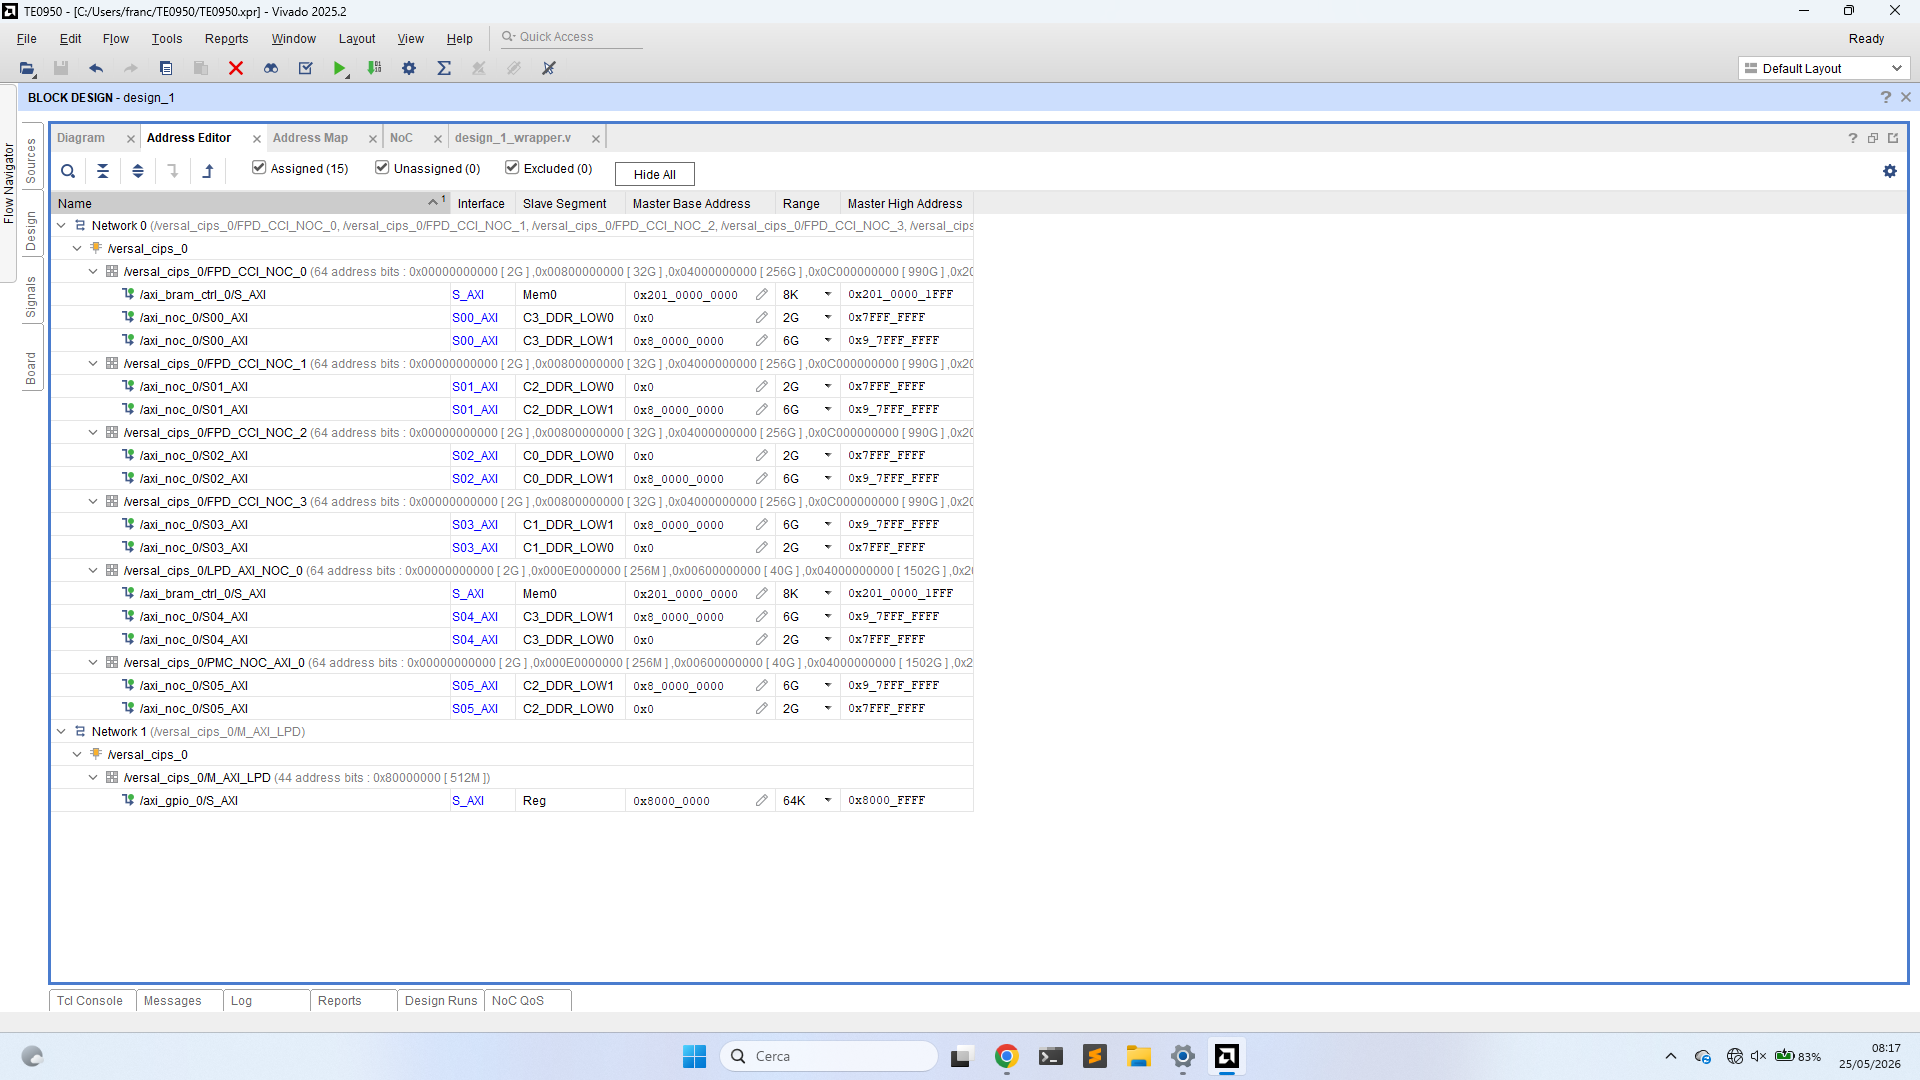
\includegraphics[width=0.85\linewidth]{Address_Editor_screenshot.png}
    \caption{Vivado Address Editor: note the \texttt{0x80000000} base address assigned to \texttt{axi\_gpio\_0} under the \texttt{M\_AXI\_LPD} master view of the CIPS.
    This address falls within the 32-bit LPD address space and is directly reachable by the Cortex-R5F.}
    \label{fig:address-editor}
\end{figure}

\paragraph*{Step 7 --- XDC pin constraints}

Create a constraints file (\textit{Sources} $\to$ \textit{Add Sources} $\to$ \textit{Add or Create Constraints}) and add the following two lines, which assign the GPIO output to the physical LED pin on the TE0950:

\begin{bashcode}
set_property PACKAGE_PIN B12 [get_ports {gpio_rtl_0_tri_o[0]}]
set_property IOSTANDARD LVCMOS33 [get_ports {gpio_rtl_0_tri_o[0]}]
\end{bashcode}

The block design should look approximately as shown below.

\begin{figure}[h]
    \centering
    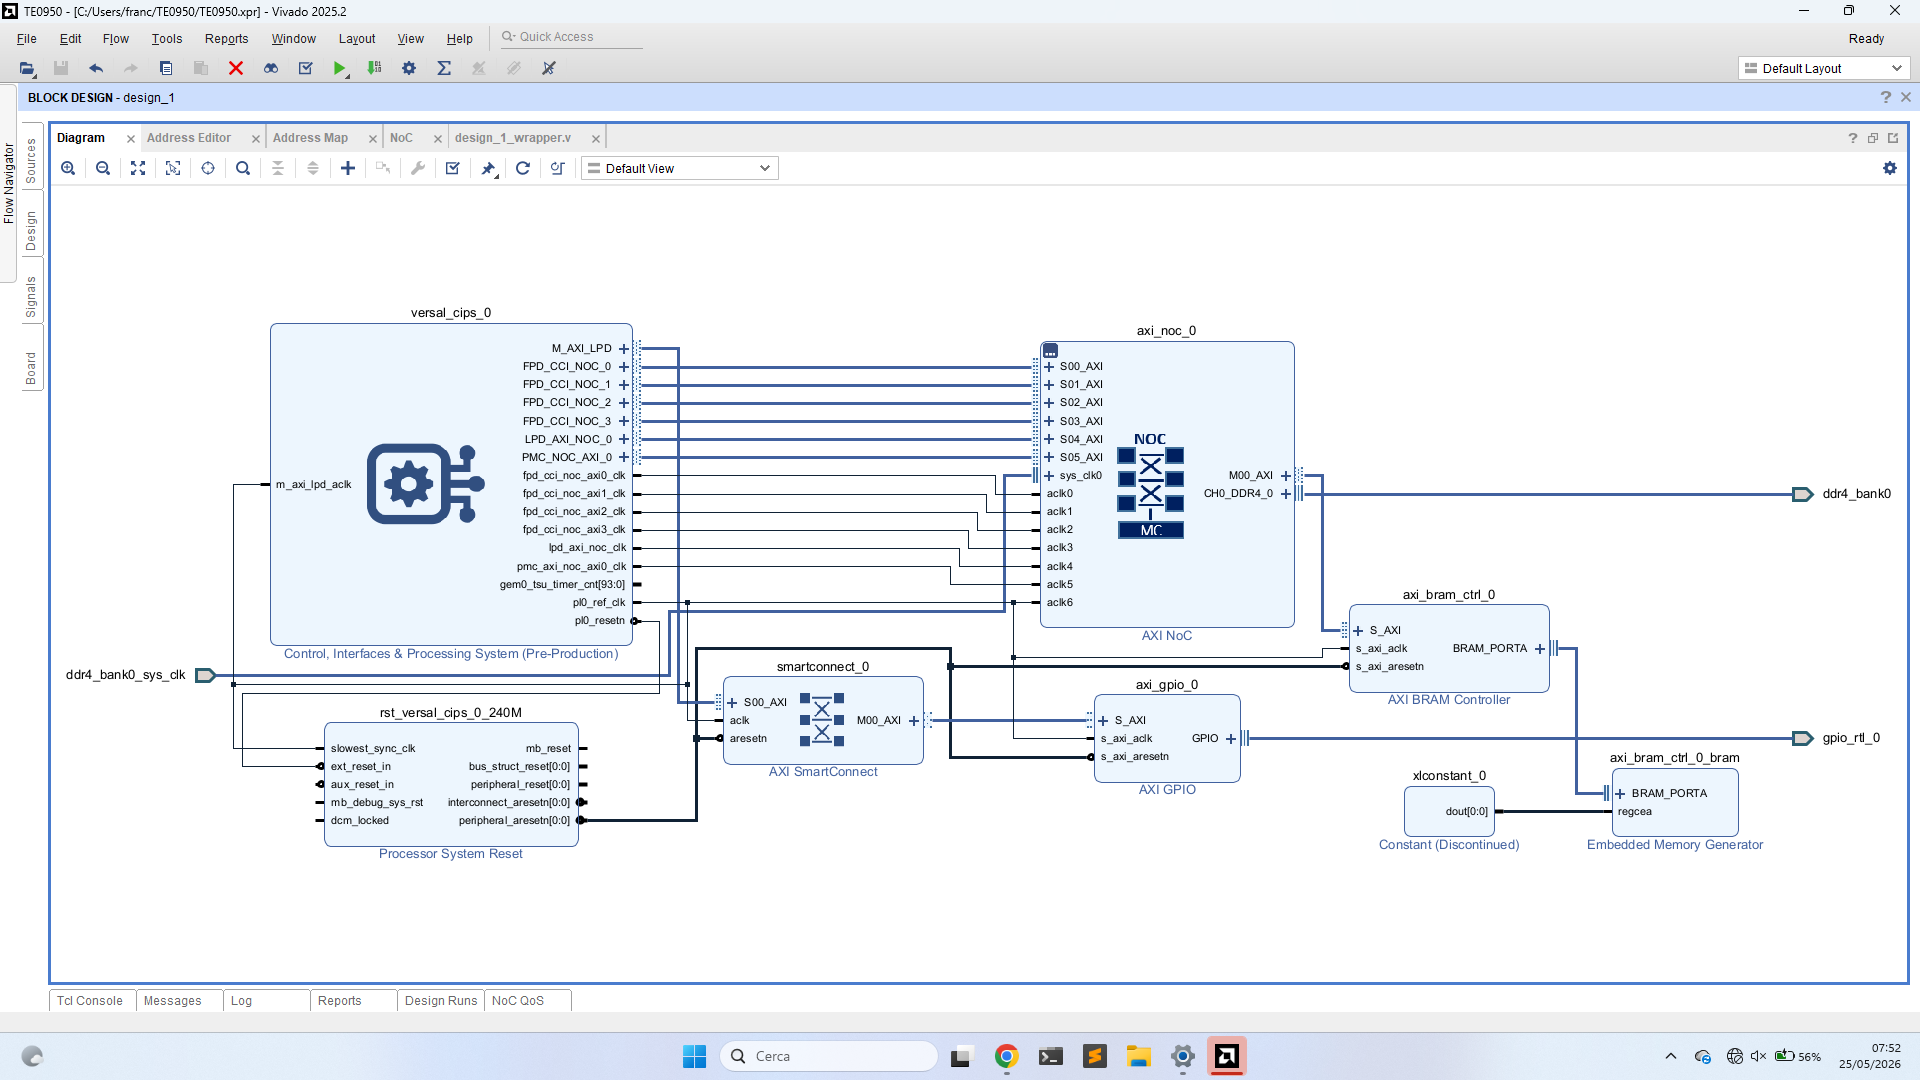
\includegraphics[width=0.85\linewidth]{TE0950_screenshot.png}
    \caption{Vivado block design after completing Steps~1--7: the CIPS \texttt{M\_AXI\_LPD} port drives the AXI SmartConnect, which in turn connects to the AXI GPIO peripheral.}
    \label{fig:vivado-block-design}
\end{figure}

\paragraph*{Step 8 --- Validate the design}

Press \texttt{F6} or select \textit{Tools} $\to$ \textit{Validate Design}.
The validation must complete with no critical errors.

\paragraph*{Step 9 --- Synthesis, implementation, and bitstream generation}

Run the full implementation flow: \textit{Generate Bitstream} from the \textit{Flow Navigator} will automatically trigger synthesis and implementation if they have not been run yet.
On Versal, this flow can take a significant amount of time; no additional intervention is required once it is launched.

\paragraph*{Step 10 --- Export XSA with bitstream}

Once bitstream generation completes, export the hardware:
\textit{File} $\to$ \textit{Export} $\to$ \textit{Export Hardware}.
In the wizard, select \textit{Include bitstream} and save the \texttt{.xsa} file to a convenient path.
This updated XSA will be imported into Vitis in the following subsection to rebuild the platform and deploy the LED application.

\subsubsection{Building and Deploying the LED Application}
\label{sec:guide-led-app}

The application build process mirrors the one described in Section~\ref{sec:guide-rtems-build} exactly: the same RTEMS toolchain, the same BSP (\texttt{arm/versal\_rpu\_split\_0}), and the same \texttt{waf}-based workflow are reused.
The only differences are the source files, the executable name, and the fact that the Vitis platform must be updated to consume the new XSA produced in the previous step before assembling the PDI.

The application directory structure is:

\begin{bashcode}
$HOME/quick-start/app/blinking_led/
  blinking_led.c   # application logic
  init.c           # RTEMS kernel configuration
  wscript          # waf build script
\end{bashcode}

\paragraph*{init.c}

The RTEMS configuration header is identical to the one used in the base application (see Section~\ref{sec:guide-rtems-build}); copy it verbatim.

\paragraph*{blinking\_led.c}

This file contains the Init task that drives the LED.
The GPIO \texttt{DATA} register is accessed through a single volatile pointer pinned to the address assigned in the Vivado Address Editor (\texttt{0x80000000}).
Writing \texttt{0x0} to that address asserts the pin low, which turns the LED on (the TE0950 user LED is active-low); writing \texttt{0x1} drives it high and turns it off.
A data synchronisation barrier (\texttt{dsb sy}) is issued after each write to ensure the store reaches the peripheral before the next sleep call.
After an initial 5-second delay (to allow the system to settle after JTAG programming), the task toggles the LED on and off every 2 seconds for ten iterations, then exits.

\begin{bashcode}
#include <rtems.h>
#include <stdint.h>
#include <string.h>
#include <stdio.h>
#include <unistd.h>

#define USR_LED_ADDR 0x80000000
#define USR_LED (* (volatile uint32_t *) USR_LED_ADDR)

#define USR_LED_ON  0x0
#define USR_LED_OFF 0x1

#define MEMORY_BARRIER __asm__ volatile ("dsb sy" ::: "memory")

void turn_led_on()  { USR_LED = USR_LED_ON;  }
void turn_led_off() { USR_LED = USR_LED_OFF; }

rtems_task Init(rtems_task_argument ignored)
{
    sleep(5);
    printf("Starting...\n");

    for (volatile uint32_t i = 0; i < 10; i++) {
        if (i % 2 == 0)
            turn_led_on();
        else
            turn_led_off();

        MEMORY_BARRIER;
        sleep(2);
    }

    printf("...exiting.\n");
    rtems_task_exit();
}
\end{bashcode}

\paragraph*{wscript}

The \texttt{wscript} is identical in structure to the one in Section~\ref{sec:guide-rtems-build}; adjust the target name and source list:

\begin{bashcode}
def build(bld):
    rtems.build(bld)
    bld(features='c cprogram',
        target='blinking_led.exe',
        source=['blinking_led.c', 'init.c'])
\end{bashcode}

\paragraph*{Configuring and building the application}

Configure and build exactly as before, pointing \texttt{waf} at the same RTEMS prefix and BSP:

\begin{bashcode}
cd $HOME/quick-start/app/blinking_led
./waf configure --rtems="$HOME/quick-start/rtems/7" \
                --rtems-bsp=arm/versal_rpu_split_0
./waf
\end{bashcode}

The compiled binary \texttt{blinking\_led.exe} is placed under \texttt{build/arm-rtems7-versal\_rpu\_split\_0/}.

\paragraph*{Updating the Vitis platform and deploying}

In Vitis, open the existing platform component (\texttt{versal\_platform}) and update its hardware source to point to the new \texttt{.xsa} exported in the previous step; then rebuild the platform.
Reassemble the PDI through \textit{Create Boot Image} as described in Section~\ref{sec:guide-vitis-base}, replacing the application ELF partition with \texttt{blinking\_led.exe}; rename it to \texttt{blinking\_led.elf} first, as Vitis may reject or mishandle the \texttt{.exe} extension when assembling the PDI.
Keep the PLM and PSM ELF entries unchanged.
Program the board with the new PDI over JTAG.
After a 5-second pause the UART console will print \texttt{Starting...}, and the user LED D1 on the TE0950 will begin toggling every 2 seconds.

%----------------------------------------------------------------------------------------
%	DEVELOPMENT PROCESS
%----------------------------------------------------------------------------------------

\section{Development Process}
\label{ch:process}

This chapter documents the practical challenges encountered during development, together with the reasoning behind the choices made to address them.
Its purpose is twofold: to give a transparent account of the decisions that shaped the final working configuration, and to serve as a reference for future developers facing similar issues on the same platform.
The chapter is divided into two parts: the first covers the work required to establish that RTEMS was actually running on the board; the second addresses the challenges encountered when extending the setup to drive the PL user LED.

%------------------------------------------------

\subsection{Verifying RTEMS Execution}
\label{sec:process-rtems}

The XSA file used throughout the entire development process is the one produced in Section~\ref{sec:guide-vivado-base}: a single hardware design was exported at the outset and reused in every subsequent step, including the bare-metal experiments described below.

The first practical obstacle was verifying whether RTEMS was running at all.
Initial attempts produced no output on the serial terminal, making it impossible to distinguish between a complete boot failure and a misconfigured console driver.
Because the team had no prior experience with the Vitis workflow, bare-metal applications were used as a stepping stone: they offer a simpler execution model, and establishing that bare-metal serial output worked correctly was a prerequisite for any further diagnosis.

\paragraph*{Bare-Metal Hello World on a Single RPU Core}

As a first step, the group reproduced the most advanced working configuration of the previous group: a single bare-metal \textit{Hello World} application running on the RPU in split mode.
This served to build familiarity with the Vitis workflow and to confirm that the hardware design and toolchain were functional.
The example project was already provided by Vitis, so it was only necessary to configure and program the board correctly.

\paragraph*{Dual-Core Bare-Metal and the Linker Script Issue}

The team then moved to running two bare-metal \textit{Hello World} applications simultaneously, one on each Cortex-R5F core.
This is where the first significant problem was encountered: each application was supposed to print ``Hello from processor~\textit{x}'' (with \textit{x} being 0 or 1), yet both cores produced the same output string.
The initial hypothesis was that the Platform Loader and Manager (PLM), that is the Versal firmware module responsible for distributing executables to the processing units and programmable logic at boot time, had loaded one executable on top of the other, causing both RPU cores to execute the same code.
This was partially confirmed by the Vitis debugger: stepping into the \texttt{printf} call on RPU\,1, the string argument was observed to be \texttt{"Hello from processor 0"} rather than the expected \texttt{"Hello from processor 1"}, indicating that RPU\,1 was executing RPU\,0's code.

Suspicion fell on the linker scripts.
Inspection revealed that both scripts specified the same load address for the \texttt{.text} section:

\begin{bashcode}
axi_noc_0_ddr_memory_DDR_LOW_0 : ORIGIN = 0x40000, LENGTH = 0x7ffc0000
\end{bashcode}

Because both executables were mapped to the same base address, the PLM overwrote the first image with the second when assembling the boot image, leaving both cores pointing to the same code in memory.
The fix was to assign non-overlapping memory regions: the first application's linker script was left unchanged, while the second was updated to:

\begin{bashcode}
axi_noc_0_ddr_memory_DDR_LOW_0 : ORIGIN = 0x10000000, LENGTH = 0x10000000
\end{bashcode}

A shared-memory region was also added in anticipation of the next experiment:

\begin{bashcode}
shared_memory : ORIGIN = 0x20000000, LENGTH = 0x00010000
\end{bashcode}

The complete linker scripts are reported in Appendix~A (\hyperref[lst:1]{Listing~1} and~\hyperref[lst:2]{2}).
After applying the fix, both applications ran correctly and printed their respective strings.

\paragraph*{Shared-Memory Validation Without RTEMS}

With dual-core bare-metal communication established, the team devised a test to determine whether RTEMS was running without relying on RTEMS serial output.
The approach was as follows: an RTEMS task would write a known value to a shared memory location, while a bare-metal application running on the other RPU core would poll that address, detect the change, and print a confirmation to the console.
This exploited the fact that bare-metal serial output had already been verified to work, thereby decoupling the question of whether RTEMS was executing from the question of whether the RTEMS console driver was configured correctly.

Before involving RTEMS, the same mechanism was validated using two bare-metal applications to confirm that the shared-memory communication itself was reliable.
The reader and writer implementations are reported in Appendix~A (\hyperref[lst:3]{Listing~3} and~\hyperref[lst:4]{4}).
Memory barriers were added manually to ensure that values written by one core were not served from a stale cache line by the other.
An alternative would have been to use the Xilinx library function that disables caching entirely; however, since that approach could not be easily replicated inside an RTEMS application, the memory barrier solution was preferred and proved sufficient.

\paragraph*{Integrating RTEMS into the Shared-Memory Test}

With the bare-metal shared-memory communication verified, the team proceeded to integrate RTEMS.
The writer application was ported to an RTEMS task (\hyperref[lst:5]{Listing~5} in Appendix~A), and a boot image was assembled in Vitis containing both that ELF and the bare-metal reader ELF.
After programming the board, however, the result matched what expected: no output was visible from the RTEMS side, and the only console activity was the polling message from the bare-metal reader.
Initial suspicion fell on the RTEMS linker scripts, but adjusting them did not resolve the issue.
Since the problem appeared to lie below the application level, the investigation escalated to lower-level debugging: rather than observing program flow alone, it became necessary to inspect registers and system state directly.
The team therefore switched to \texttt{xsdb}, the command-line debugger integrated into the Vitis toolchain.
A natural diagnostic approach at this point was to read the UART and timer registers directly via \texttt{xsdb}, as their state could distinguish between two failure modes: RTEMS halting before any meaningful execution, versus RTEMS running normally but producing no visible output.

\paragraph*{Low-Level Debugging with XSDB}

Reading the UART registers via \texttt{xsdb} revealed that UART0 had not been initialised.
Sampling the program counter (PC) repeatedly showed it frozen at the same address across all reads, confirming that the CPU was not making progress.
Using \texttt{addr2line} to resolve that address to a source location pinpointed the exact point of failure: RTEMS was spinning inside the UART0 initialisation routine, waiting for the transmit FIFO to drain before enabling the peripheral.
Because UART0 had never been enabled by the hardware, the FIFO could not become empty, and the spin-wait never terminated.

As a first step to confirm the root cause, the spin-wait was commented out so that RTEMS could complete its initialisation and proceed without a correctly configured UART.
With that change in place, the bare-metal reader successfully detected the sentinel value written to shared memory by the RTEMS writer task, confirming that RTEMS itself was fully operational and that the only problem was the UART initialisation.

\paragraph*{Restoring Serial Output}

Rather than debugging the high-level \texttt{printf} path immediately, the team first bypassed the C library entirely and wrote characters directly to the UART data register.
This approach allowed the peripheral itself to be verified as reachable before involving the RTEMS console driver.
Both UART0 (base address \texttt{0xFF000000}) and UART1 (base address \texttt{0xFF010000}) were tested using a \texttt{custom\_printf} helper that polls the transmit-FIFO-full flag and writes one byte at a time; the implementation is reported in Appendix~A (\hyperref[lst:6]{Listing~6}).
Direct writes to UART1 produced visible output, while the same test on UART0 did not.

Inspecting the RTEMS BSP source revealed the root cause: the BSP defaults the console to minor device~0, which maps to UART0.
Because the Versal hardware does not initialise UART0, the driver cannot configure it and console output is silently lost.
The fix was a single addition to \texttt{config.ini}:

\begin{bashcode}
BSP_CONSOLE_MINOR = 1
\end{bashcode}

This redirects the RTEMS console to UART1.
After recompiling RTEMS with this setting, the original application code using standard \texttt{printf} worked correctly without any further changes.

\begin{quote}
\textbf{Note.}
UART0 could have been enabled as an alternative path: in Vivado, opening the CIPS configuration dialog and navigating to \textit{PS PMC} $\to$ \textit{Peripherals} $\to$ \textit{UART} allows UART0 to be activated and assigned to its default MIO pin pair.
Doing so would have allowed the BSP default (minor device~0) to work without any change to \texttt{config.ini}.
The \texttt{BSP\_CONSOLE\_MINOR = 1} approach was retained because it required no hardware redesign and the XSA had already been finalised.
\end{quote}

%------------------------------------------------

\subsection{LED Blink Debugging}
\label{sec:process-led}

The most significant challenges in this part of the project were encountered in the Vivado hardware design phase.
While the base Vivado design followed an existing online guide, no equivalent resource was found for adding an AXI GPIO peripheral connected to the user LED, so the necessary block design modifications were worked out independently.

\paragraph*{NoC Address Space Issue}

The first major obstacle arose when trying to route the GPIO peripheral through the AXI NoC.
In the Vivado Address Editor, all addresses automatically assigned to the GPIO via the NoC fell above the 4\,GB boundary, placing them outside the 32-bit address space of the RPU.
Since the Cortex-R5F cannot issue memory transactions to addresses above \texttt{0xFFFFFFFF}, these assignments were unusable.
The solution was to bypass the NoC master port entirely and connect the LPD AXI port of the CIPS directly to an AXI SmartConnect, which in turn drives the GPIO peripheral.
This path stays within the 32-bit LPD address space and allows the address to be assigned at \texttt{0x80000000}, reachable by the RPU.

\paragraph*{Bare-Metal Validation}

Once the XSA was correctly exported with the GPIO peripheral mapped at \texttt{0x80000000}, the design was first validated with a bare-metal application.
The LED toggled as expected, confirming that the Vivado design, the XDC pin constraints, and the address assignment were all correct.

\paragraph*{RTEMS Crash and MPU Fix}

Replacing the bare-metal application with the RTEMS blinking-LED application (\hyperref[lst:7]{Listing~7} in Appendix~A) caused an immediate crash.
The most likely cause was that the memory region containing the GPIO address was not covered by any MPU region in the RTEMS BSP: on the Cortex-R5F, any access to a region not explicitly enabled in the MPU triggers a fault, regardless of whether the address is physically valid.
The fix was to add the following entry to the MPU table in \texttt{bsps/arm/versal\_rpu/start/bspstart.c}:

\begin{bashcode}
{
  .begin = 0xFFE00000U,
  .end   = 0xFFEFFFFFU,
  .rasr  = ARMV7_MPU_RASR_XN |
           ARMV7_MPU_RASR_AP(0x3) |
           ARMV7_MPU_RASR_TEX_1_S(0x0) |
           ARMV7_MPU_RASR_SIZE(0x13) |
           ARMV7_MPU_RASR_ENABLE
},
\end{bashcode}

This entry covers the 1\,MB region \texttt{0xFFE00000}--\texttt{0xFFEFFFFF} and configures it as Device memory (non-cacheable, non-bufferable) with full read/write access and the Execute Never flag set.
After recompiling RTEMS with this addition and programming the board, the application ran correctly and the LED blinked as expected.


%----------------------------------------------------------------------------------------
%	APPENDIX
%----------------------------------------------------------------------------------------

\appendix

\section{Source Listings}
\label{app:listings}

The listings below reproduce the source files referenced in Section~\ref{ch:process}.
Listings~1 and~2 are the linker scripts for the writer (RPU\,0) and reader (RPU\,1) bare-metal applications; the sole differences between them are the base address and size of the DDR region and the inclusion of the shared-memory region.

\phantomsection\label{lst:1}
\begin{appendixcode}{Listing 1 --- Writer linker script (\texttt{lscript\_writer.ld}, RPU\,0)}
\lstinputlisting{src/lscript_writer.ld}
\end{appendixcode}

\phantomsection\label{lst:2}
\begin{appendixcode}{Listing 2 --- Reader linker script (\texttt{lscript\_reader.ld}, RPU\,1)}
\lstinputlisting{src/lscript_reader.ld}
\end{appendixcode}

\phantomsection\label{lst:3}
\begin{appendixcode}{Listing 3 --- Bare-metal writer (\texttt{writer.c}, RPU\,0)}
\lstinputlisting{src/writer.c}
\end{appendixcode}

\phantomsection\label{lst:4}
\begin{appendixcode}{Listing 4 --- Bare-metal reader (\texttt{reader.c}, RPU\,1)}
\lstinputlisting{src/reader.c}
\end{appendixcode}

\phantomsection\label{lst:5}
\begin{appendixcode}{Listing 5 --- RTEMS writer task (\texttt{rtems\_init.c})}
\lstinputlisting{src/rtems_init.c}
\end{appendixcode}

\phantomsection\label{lst:6}
\begin{appendixcode}{Listing 6 --- RTEMS writer with direct UART access (\texttt{rtems\_init\_uart.c})}
\lstinputlisting{src/rtems_init_uart.c}
\end{appendixcode}

\phantomsection\label{lst:7}
\begin{appendixcode}{Listing 7 --- RTEMS blinking-LED application (\texttt{blinking\_led.c})}
\lstinputlisting{src/blinking_led.c}
\end{appendixcode}

%----------------------------------------------------------------------------------------
%	REFERENCES
%----------------------------------------------------------------------------------------

\printbibliography[title={References}]

%----------------------------------------------------------------------------------------

\end{document}
